\documentclass[10pt, landscape]{article}
\usepackage[scaled=0.92]{helvet}
\usepackage{calc}
\usepackage{multicol}
\usepackage{ifthen}
\usepackage[a4paper,margin=3mm,landscape]{geometry}
\usepackage{amsmath,amsthm,amsfonts,amssymb}
\usepackage{color,graphicx,overpic}
\usepackage{hyperref}
\usepackage{newtxtext} 
\usepackage{enumitem}
\usepackage{amssymb}
\usepackage[table]{xcolor}
\usepackage{vwcol}
\usepackage{tikz}
\usetikzlibrary{arrows.meta}
\usetikzlibrary{calc}
\usepackage{mathtools}
\usepackage{nicematrix}
%For pictures / figures
\usepackage{color,graphicx,overpic}
\graphicspath{ {./images/midterm/} }
% for relations
\usepackage{cancel}
\usepackage{ mathrsfs }
\graphicspath{ {./images/} }
\setlist{nosep}
\usepackage{amssymb}  % For \checkmark


\pdfinfo{
  /Title (EE3408C-Midterm-Cheatsheet.pdf)
  /Creator (TeX)
  /Producer (pdfTeX 1.40.0)
  /Author (Seamus)
  /Subject (Example)
  /Keywords (pdflatex, latex,pdftex,tex)}

% Turn off header and footer
\pagestyle{empty}

\newenvironment{tightcenter}{%
  \setlength\topsep{0pt}
  \setlength\parskip{0pt}
  \begin{center}
}{%
  \end{center}
}

% redefine section commands to use less space
\makeatletter
\renewcommand{\section}{\@startsection{section}{1}{0mm}%
                                {-1ex plus -.5ex minus -.2ex}%
                                {0.5ex plus .2ex}%x
                                {\normalfont\large\bfseries}}
\renewcommand{\subsection}{\@startsection{subsection}{2}{0mm}%
                                {-1explus -.5ex minus -.2ex}%
                                {0.5ex plus .2ex}%
                                {\normalfont\normalsize\bfseries}}
\renewcommand{\subsubsection}{\@startsection{subsubsection}{3}{0mm}%
                                {-1ex plus -.5ex minus -.2ex}%
                                {1ex plus .2ex}%
                                {\normalfont\small\bfseries}}%
\renewcommand{\familydefault}{\sfdefault}
\renewcommand\rmdefault{\sfdefault}
% makes nested numbering (e.g. 1.1.1, 1.1.2, etc)
\renewcommand{\labelenumii}{\theenumii}
\renewcommand{\theenumii}{\theenumi.\arabic{enumii}.}
\renewcommand\labelitemii{•}
%  for logical not operator
\renewcommand{\lnot}{\mathord{\sim}}
\renewcommand{\bf}[1]{\textbf{#1}}
\newcommand{\abs}[1]{\vert #1 \vert}
\newcommand{\Mod}[1]{\ \mathrm{mod}\ #1}

\makeatother
\definecolor{myblue}{cmyk}{1,.72,0,.38}
\everymath\expandafter{\the\everymath \color{myblue}}
% Define BibTeX command
\def\BibTeX{{\rm B\kern-.05em{\sc i\kern-.025em b}\kern-.08em
    T\kern-.1667em\lower.7ex\hbox{E}\kern-.125emX}}
\let\iff\leftrightarrow
\let\Iff\Leftrightarrow
\let\then\rightarrow
\let\Then\Rightarrow

% Don't print section numbers
\setcounter{secnumdepth}{0}

\setlength{\parindent}{0pt}
\setlength{\parskip}{0pt plus 0.5ex}
%% this changes all items (enumerate and itemize)
\setlength{\leftmargini}{0.5cm}
\setlength{\leftmarginii}{0.5cm}
\setlist[itemize,1]{leftmargin=2mm,labelindent=1mm,labelsep=1mm}
\setlist[itemize,2]{leftmargin=4mm,labelindent=1mm,labelsep=1mm}

%My Environments
\newtheorem{example}[section]{Example}
% -----------------------------------------------------------------------

\begin{document}
\raggedright
\footnotesize
\begin{multicols}{4}


% multicol parameters
% These lengths are set only within the two main columns
\setlength{\columnseprule}{0.25pt}
\setlength{\premulticols}{1pt}
\setlength{\postmulticols}{1pt}
\setlength{\multicolsep}{1pt}
\setlength{\columnsep}{2pt}

\begin{center}
    \fbox{%
        \parbox{0.8\linewidth}{\centering \textcolor{black}{
            {\Large\textbf{EE3408C Final}}
            \\ \normalsize{AY26/27 sem 1}}
            \\ {\footnotesize \textcolor{myblue}{github.com/mendax1234}} 
        }%
    }
\end{center}

\section{Review of Basic MOSFETs}
% TODO: Add the symbol of NMOS and PMOS by hand after printing this cheatsheet
% TODO: Know the amplitude and magnitude of the signal (meaning)
\begin{enumerate}
    \item (\textbf{Triode Region}) NMOS in triode region, the drain current equation is
    $$I_D = \mu_n C_{ox} \frac{W}{L}\left[(V_{GS} - V_{TH})V_{DS} - \frac{1}{2}V_{DS}^2\right]$$
    If $V_{DS} \ll 2(V_{GS} - V_{TH})$, which is the same as $\frac{1}{2}V_{DS}^2 \ll (V_{GS} - V_{TH})V_{DS}$, the drain current equation can be simplified to
    $$I_D \approx \mu_n C_{ox} \frac{W}{L} (V_{GS} - V_{TH}) V_{DS}$$
    Thus, the NMOS behaves like a resistor and its on resistance is
    $$R_{on} = \frac{V_{DS}}{I_D} = \frac{1}{\mu_n C_{ox} \frac{W}{L} (V_{GS} - V_{TH})}$$
    For PMOS, the drain current is
    $$|I_D| = \mu_p C_{ox} \frac{W}{L} \left[ \left( V_{SG} - |V_{THP}| \right) V_{SD} - \frac{1}{2} V_{SD}^2 \right]$$
    \item $k_n'=\mu_nC_{OX}$ ,$V_{OV}=V_{GS}-V_{THN}$
    \item (\textbf{Saturation Region}): When NMOS operates in saturation region, its drain current is
    $$ I_D = \frac{1}{2}\mu_n C_{ox} \frac{W}{L} (V_{GS} - V_{TH})^2$$
    For PMOS, the drain current is
    $$I_D = -\frac{1}{2}\mu_p C_{ox} \frac{W}{L} (V_{GS} - V_{TH})^2$$
    \item (\textbf{NMOS Operation Region Quick Check}):\\
    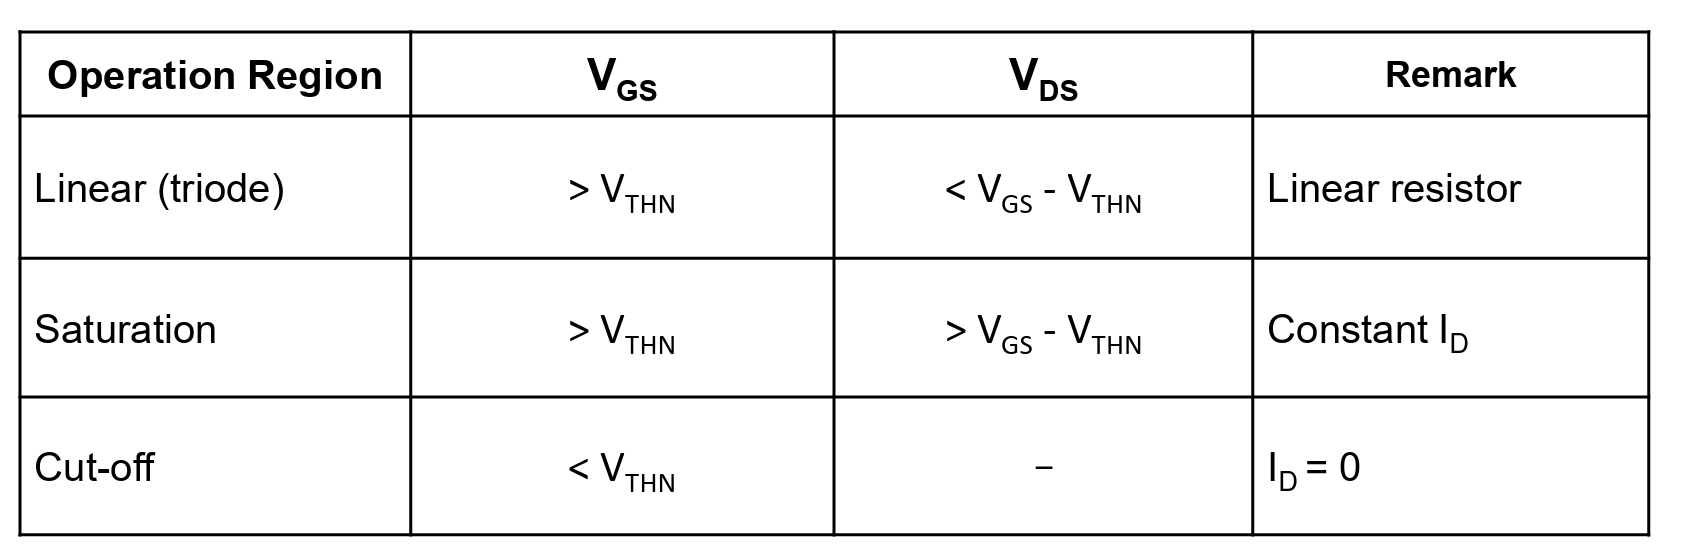
\includegraphics[width=1\linewidth]{images/final/1.png}
    \item (\textbf{PMOS Operation Region Quick Check}):\\
    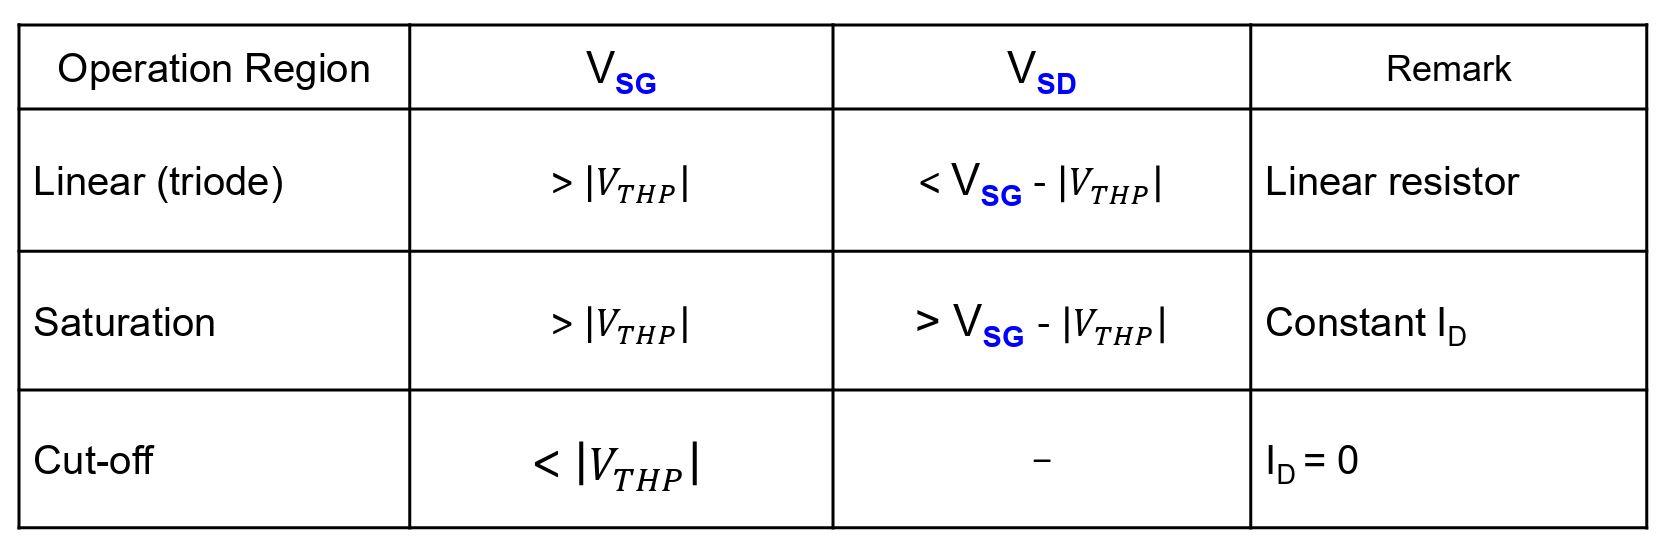
\includegraphics[width=1\linewidth]{images/final/2.png}
    \item For MOSFET to work under \textbf{saturation}, a quick check is to check if $V_{SD\text{(PMOS)}/DS\text{(NMOS)}}\geq V_{OV}$
    \item \textbf{MOSFET Saturation Check}:
    \begin{itemize}
        \item (Cadence Virtuoso Method): Both NMOS and PMOS operate in saturation when $|V_{DS}| \geq |V_{DSAT}|$ where $|V_{DSAT}|=V_{GS}-V_{THN}\text{ or }V_{SG}-|V_{THP}|$ denotes the minimum $V_{DS}$ necessary for operation in saturation.
        \item (Inspired by ``pinch-off''): Assuming the MOSFET is turned on, saturation can also be checked without knowing the source voltage: $V_{GD}\leq V_{THN}$ (NMOS) or $V_{DG}\leq |V_{THP}|$ (PMOS).
    \end{itemize}
    \item (\textbf{Transconductance}): The definition of transconductance $g_m$ is given below, which holds in both saturation and linear region. (Unit is \textbf{S})
    $$g_m = \left. \frac{\partial I_D}{\partial V_{GS}} \right|_{V_{DS,\text{const.}}}$$
    \begin{itemize}
        \item \textbf{Saturation Region}
        \begin{itemize}
            \item For NMOS operating in \textbf{saturation region}, $g_m = \mu_n C_{ox} \frac{W}{L} (V_{GS} - V_{TH}) = \sqrt{2 \mu_n C_{ox} \frac{W}{L} I_D}= \frac{2 I_D}{V_{GS} - V_{TH}}$
            \item For PMOS operating in \textbf{saturation region}, $g_m = \mu_p C_{ox}\frac{W}{L}(V_{SG}-|V_{THP}|) = \sqrt{2\mu_p C_{ox}\frac{W}{L}I_D}=\frac{2I_D}{V_{SG}-|V_{THP}|}$
            \item If we consider CLM, we will just times the first and second equation with $1+\lambda V_{\text{DS}}$ (the second will be in the square root), while the third equation remains unchanged.
        \end{itemize}
        \item (\textbf{Linear Region}): For NMOS operating in \textbf{linear region}, its $g_m$ is $g_m=\mu_n C_{ox} \frac{W}{L} V_{DS}$. For PMOS, just replace $V_{DS}$ with $V_{SD}$
    \end{itemize}
    \item (\textbf{Body Effect}): In body effect, the threshold voltage for NMOS is redefined to be
    $$
    V_{THn} = V_{TH0} + \gamma \left( \sqrt{2\Phi_F + V_{SB}} - \sqrt{|2\Phi_F|} \right)
    $$
    while in PMOS, it is
    $$\vert{}V_{THp}\vert{} = \vert{}V_{TH0p}\vert{} + \gamma (\sqrt{\vert{}2\Phi_F\vert{} + V_{BS}} - \sqrt{\vert{}2\Phi_F\vert{}})$$
    For the body effect, we should understand the following 2 trends
    \begin{itemize}
        \item NMOS: $V_{SB}\uparrow \text{or } V_{BS}<0\Rightarrow V_{TH}\uparrow\Rightarrow I_D\downarrow$
        \item PMOS: $V_{BS}\uparrow \text{or } V_{BS}>0\Rightarrow |V_{THP}|\uparrow\Rightarrow I_D\downarrow$
        \item $V_{BS}=0$, no body effect.
        \item \textbf{When to consider body effect:} The body of an \textbf{NMOS} is typically connected to \textbf{GND}, while the body of a \textbf{PMOS} is typically connected to $V_{DD}$. Then check the source voltage, if the body-to-source voltage varies ($v_{bs}\neq 0$), include $g_{mb}v_{bs}$ in small-signal model.
    \end{itemize}
    \item (\textbf{Channel Length Modulation}): If the question explicitly says considering CLM, we should consider CLM, otherwise, don't consider. If consider CLM, the drain current when a NMOS operates in saturation region is (CLM doesn't exist in triode region):
    $$I_D \approx \frac{1}{2}\mu_n C_{ox}\frac{W}{L}(V_{GS}-V_{TH})^2(1+\lambda V_{DS})$$
    In EE3408C, we won't consider CLM in transconductance calculation, but \textbf{will consider that in small signal analysis, e.g., to calculate the output resistance}.
    \item Strong inversion region is usually the \textbf{same as} saturation region.
\end{enumerate}

\section{MOSFET Small-Signal Model}
\begin{enumerate}
    \item (\textbf{NMOS Small Signal Model}):
    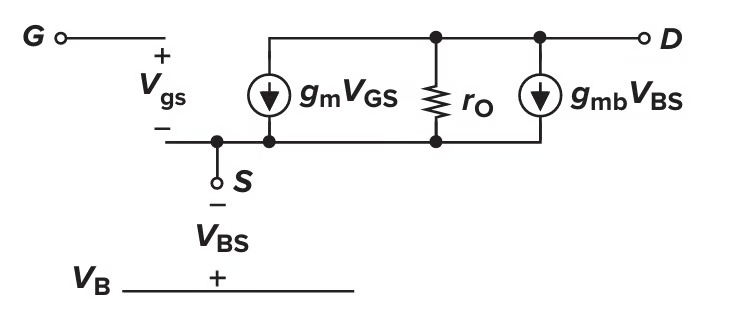
\includegraphics[width=1\linewidth]{images/midterm/2.png}
    \item (\textbf{PMOS Small Signal Model}):
    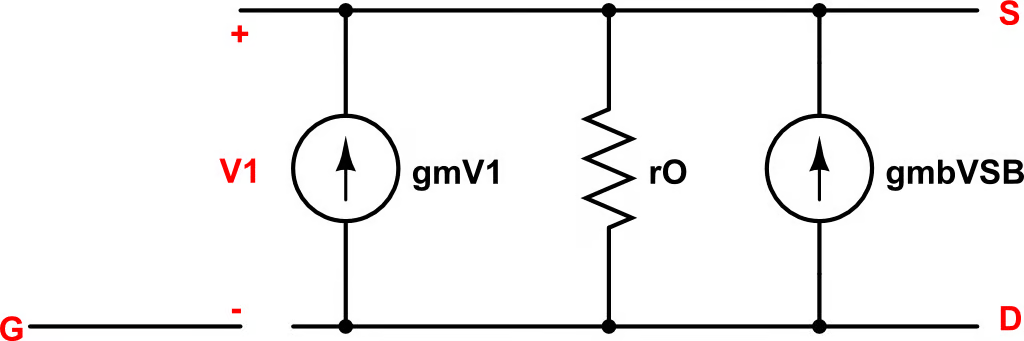
\includegraphics[width=1\linewidth]{images/midterm/3.png}
    \item In the \textbf{MOSFET small-signal model}, $g_{mb}=\eta g_m$, where $\eta=\frac{\partial V_{THN}}{\partial V_{SB}}$ (NMOS) or $\eta=\frac{\partial |V_{THP}|}{\partial V_{BS}}$ (PMOS) is the \textbf{body-effect factor}, typically approximated as $0.25$.
    \item In the MOS Small signal model, the output resistance only exists if we consider the CLM, and its value is $r_o\approx \frac{1}{\lambda I_D}$. Its definition formula is $r_o=\frac{\partial V_{DS}}{\partial I_D}$
    \item (\textbf{MOS Capacitance}): Define the gate-channel and overlap capacitances: $C_{GC} = WLC_{ox},C_{GS0} = C_{GD0} = C_{ov}W$
    \begin{itemize}
        \item \textbf{Cut-off region:}
        $
        C_{GS} = C_{GS0},
        C_{GD} = C_{GD0},
        C_{GB} = \frac{C_{GC}C_d}{C_{GC}+C_d}
        $
        \item \textbf{Triode region:} $C_{GC}$ is approximately equally divided between the source and drain.
        $
        C_{GS} = C_{GD} = C_{GS0} + \frac{1}{2}WLC_{ox},
        C_{GB} = 0
        $
        \item \textbf{Saturation region:} the drain side is depleted, so approximately $\frac{2}{3}C_{GC}$ appears at the source side.
        $
        C_{GS} = C_{GS0} + \frac{2}{3}WLC_{ox},
        C_{GD} = C_{GD0},
        C_{GB} = 0
        $
    \end{itemize}
    \item \textbf{Miscs}
    \begin{itemize}
        \item When the question asks how one thing changes with the other thing, we do \textbf{partial differentiation} to find the change rate using the given values!
        \item \textbf{Useful MOS amplifier approximations:} $g_m\approx 2\,\mathrm{mS}$ ($1/g_m\approx 500\,\Omega$), $r_o\approx 200\,\mathrm{k}\Omega$, $R_D\approx 5\,\mathrm{k}\Omega$, $R_{\mathrm{load}}\approx 100\,\mathrm{k}\Omega$ (using MOSFET instead of normal resistors as the load), and $g_{mb}\approx 0.1g_m$\text{ to }$0.3g_m$. 
    \end{itemize}
\end{enumerate}

\section{Single-Stage Amplifier Design}
\begin{enumerate}
    \item Intuitive Small-Signal Analysis: This is to quickly get the voltage gain of any analog circuit.
    \begin{itemize}
        \item Find the output resistance $R_{\text{out}}$ of the circuit.
        \item Find the equivalent $G_M$ of the circuit.
        \item Calculate the voltage gain using $A_V=-G_M\times R_{\text{out}}$ (If not sure, just use absolute voltage gain in the exam)
    \end{itemize}
    \item Find the output resistance $R_{\text{out}}$ of the circuit: Usually we have two methods.
    \begin{enumerate}
        \item The intuitive shortcut (Suitable for most cases): \\
        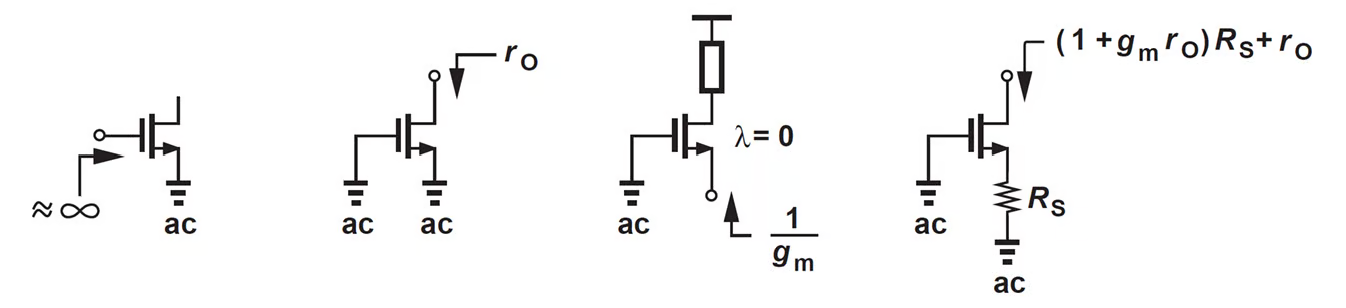
\includegraphics[width=1\linewidth]{images/midterm/4.png}
        \begin{itemize}
            \item In the third case, no matter what is connected at the drain, the resistance looking from the source terminal is always $\frac{1}{g_m}$.
            \item In the fourth case, we usually just use the approximation of $g_mr_oR_S$
            \item For a diode-connected MOSFET (gate and drain are connected together), its impedance is always $\frac{1}{g_m}$ (from both the view of source and drain) if we ignore the body effect.
            \item For pure NMOS and PMOS without any load, looking into the \textbf{drain terminal} gives us a resistance of $r_o$. Looking into the \textbf{source terminal} gives us a resistance of $\frac{1}{g_m}$.
        \end{itemize}
        \item Thevenin Equivalent (Test-voltage method):
        \begin{center}
            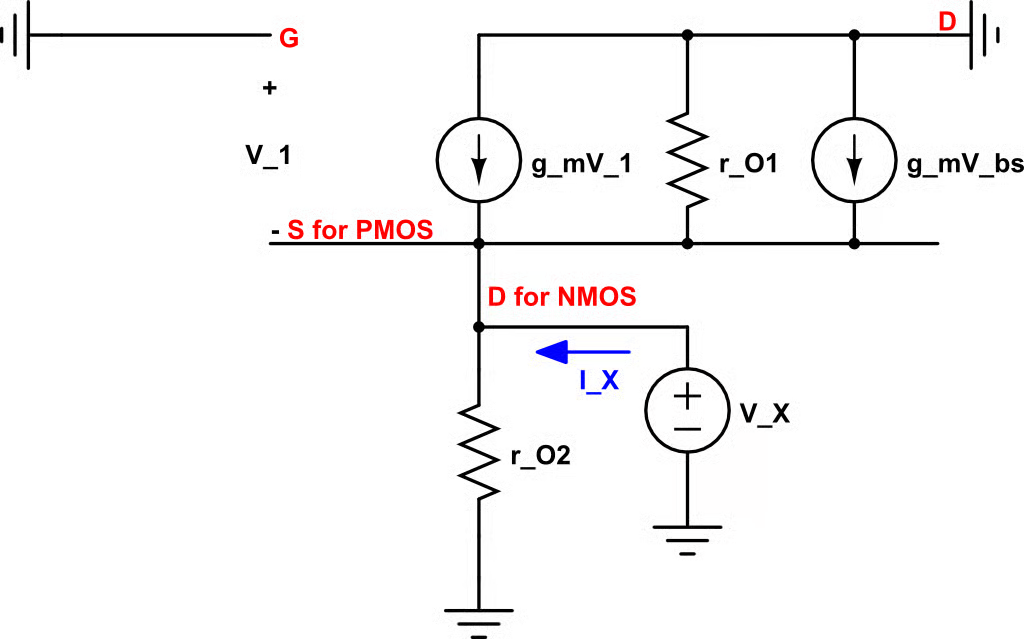
\includegraphics[width=0.8\linewidth]{images/final/3.png}
        \end{center}
        \begin{itemize}
            \item Add a test-voltage source at the node we want to look into. (Suppose the voltage source's voltage $V_X$ is given)
            \item Treat all the \textbf{independent voltage sources} as \textbf{AC ground} and \textbf{independent current sources} as open circuit. (Most sources we will encounter in this mod are independent voltage sources!)
            \item Measure the current $I_X$ flowing into the node. (Use KCL during the exam)
            \item Solve for $R_{\text{out}}=\frac{V_X}{I_X}$.
        \end{itemize}
        \item For three arbitrary resistors $R_A$, $R_B$, and $R_C$ in \textbf{parallel}, their equivalent resistance is $R_A \parallel R_B \parallel R_C = \frac{1}{\frac{1}{R_A}+\frac{1}{R_B}+\frac{1}{R_C}}$.
        \item For resistors in \textbf{parallel}, the equivalent resistance is approximately the \textbf{smallest resistance} if the other resistances are much larger. For example, if $R_A \gg R_B$, then $R_A \parallel R_B \approx R_B$. Similarly, if $R_A \gg R_B, R_C$, then $R_A \parallel R_B \parallel R_C \approx R_B \parallel R_C$.
    \end{enumerate}
    \item Find the equivalent $G_M$ of the circuit
    \begin{enumerate}
        \item Common transconductance in the circuit level:
        \begin{itemize}
            \item In a single-stage CS amplifier where the input is at the \textbf{gate} terminal, the output is at the \textbf{drain} terminal of the NMOS M1 and the source is connected to an AC ground, $G_m=g_{m1}$.
            \item In a single-stage CD amplifier (Source follower) where the input is at the \textbf{gate} terminal and the output is at the \textbf{source} terminal of the NMOS M1, $G_m=g_{m1}$.
            \item In a single-stage CG amplifier where the gate is connected to an AC ground, the input is at the \textbf{source} terminal and the output is at the \textbf{drain} terminal of teh NMOS M1, $G_m=-g_{m1}$.
            \item In a cascode stage amplifier, basically 2-stage amplifier (CS + CG), we usually calculate the final $G_m$ by separating the stage
            \begin{center}
                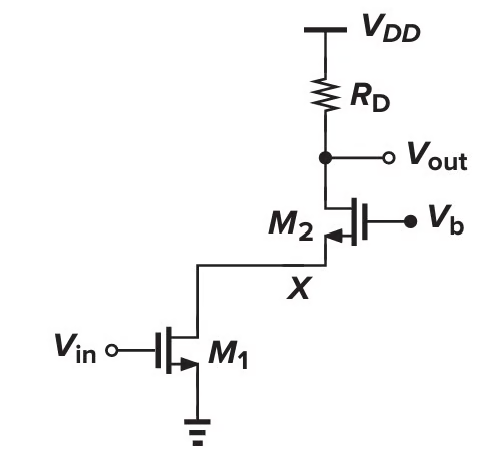
\includegraphics[width=0.5\linewidth]{images/midterm/5.png}
            \end{center}
            So, $G_m=\frac{i_{out}}{v_{in}}=\frac{i_{out}}{v_{x}}\times\frac{v_{x}}{v_{in}}$. And we can use the similar method to find the voltage gain of the first-stage and use our faster conclusions to find the $G_m'$ of the second stage ($-g_{m2}$). Thus, find the $G_m$ of the whole stage! As a shortcut, if the output is connect to drain terminal of NMOS M2, $G_m=g_{m1}$
        \end{itemize}
        \item The hand calculation method
        \begin{center}
            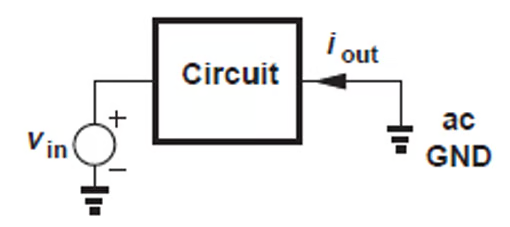
\includegraphics[width=0.6\linewidth]{images/final/4.png}
        \end{center}
        \begin{itemize}
            \item We set $v_{\text{out}}=0$ to mimic the condition when we define the transconductance in a MOS device, which is when $V_{\text{DS}}=\text{const}$. (Set the output node to AC ground)
            \item Suppose we already know $v_{\text{in}}$, we then measure the $i_{\text{out}}$ \textbf{flowing into} the circuit (The current should always flow into the circuit, and in the exams instead of measuring, we use KCL to calculate).
            \item $G_M=\frac{i_\text{out}}{v_{in}}$
        \end{itemize}
    \end{enumerate}
    \item Intuitive Understanding of each type of amplifier:
    \begin{itemize}
        \item The CS amplifier is used to amplify the input signal, but in an \textbf{inverting} manner.
        \item The CD amplifier (source follower) is used to pass the voltage at its input to its output with small loss, thus its $A_v\approx 1$.
        \item The CG amplifier is used to \textbf{amplify the input signal} (or provide \textbf{low input resistance}) while producing a non-inverted voltage output.
        \item The cascode amplifier combines a \textbf{CS stage and a CG stage}: the CS transistor converts the input voltage into a signal current, while the CG transistor keeps the CS transistor's drain voltage relatively constant. Thus, it provides \textbf{high voltage gain} by achieving a large output resistance while retaining the transconductance of the CS stage.
    \end{itemize}
\end{enumerate}

\section{Frequency Response Part 1}
\begin{enumerate}
    \item \textbf{Big picture}: In the frequency response, we are more interested in writing out the transfer function of our analog circuit, which is $H(s)=\frac{V_{\text{out}}(s)}{V_{\text{in}}(s)}=A_v\times\frac{(1-s/z_1)(1-s/z_2)\cdots}{(1+s/\omega_1)(1+s/\omega_2)(1+s/\omega_3)\cdots}$. (The zeros and poles here should be in the unit of rad/s). To do so, we need to find the 3 key components in this transfer function.
    \begin{itemize}
        \item \textbf{Voltage gain}: $A_v$. This can be found using the intuitive analysis introduced earlier!
        \item \textbf{Poles}: Use the technique of association of poles!
        \item \textbf{Zeros}: Use the quick technique we will introduce later!
    \end{itemize}
    After writing out the transfer function, we can use the general rules to draw the bode plot of our analog circuit.
    \item (\textbf{Miller Theorem}): This theorem might be performed before we draw the circuit for association of poles. In the following circuit, $C_1=C(1-A_v)$ and $C_2=C(1-\frac{1}{A_v})$ \\
    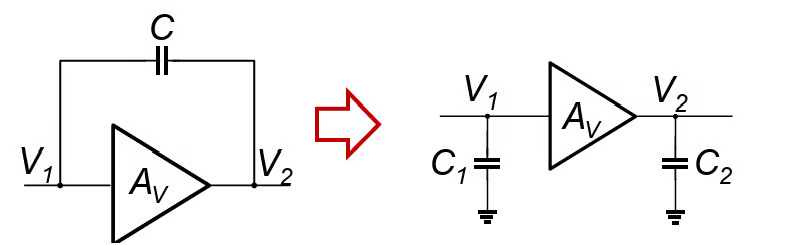
\includegraphics[width=1\linewidth]{images/midterm/6.png}
    \item (\textbf{Association of Poles}):
    \begin{itemize}
        \item When using the rule of association of poles, it suffices if we just draw the circuit diagram like below (not necessarily the small-signal circuit) and write out the \textbf{number of nodes}! \\
        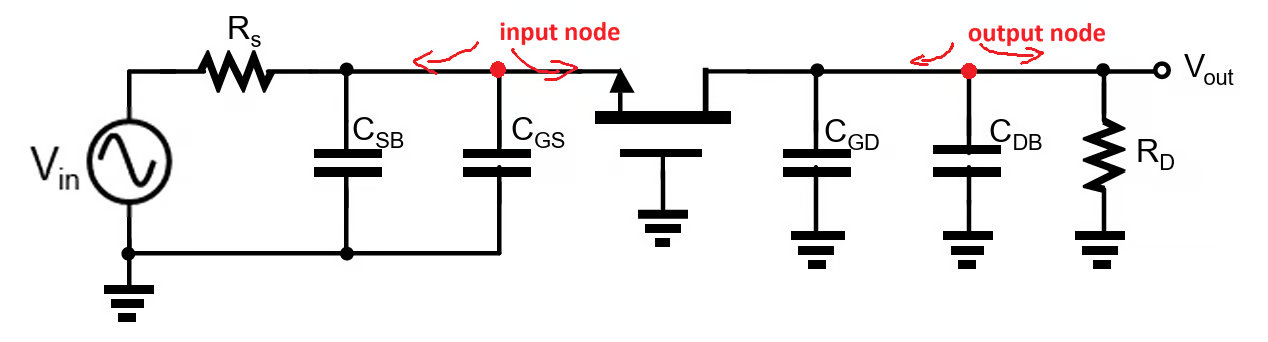
\includegraphics[width=1\linewidth]{images/midterm/7.png}
        \item When constructing a diagram as such, we treat $V_{DD}$ and $V_{in}$ as AC ground. And only draw the parasitic capacitances that are given in the question! If not given, ignore them!
        \item The number of \textbf{poles} in a circuit is equal to the number of \textbf{high-impedance nodes} in the circuit. (An input node with no resistance associated with it is not counted as a high-impedence node).
        \item \textbf{Calculate the pole frequency}:
        \begin{itemize}
            \item Find $R_{\text{eq}}$: the equivalent resistance seen looking into the node, with \textbf{independent sources set to zero} and \textbf{capacitors open-circuited}. When the node has two branches, the equivalent resistance is: $R_{\text{eq}}=R_{\text{eq,left}}\parallel R_{\text{eq,right}}$.
            \item Find $C_{\text{eq}}$: the total capacitance connected between that node and \textbf{AC ground}. (Treat the MOS as an open circuit and ignore all the resistors)!
            \item Estimate the associated pole using $\omega_p\approx\frac{1}{R_{\text{eq}}C_{\text{eq}}}$. The unit is in \textbf{rad/s} and needs to convert to Hz by dividing $2\pi$.
        \end{itemize}
        \item As in EE3408C, we are only dealing with circuits with positive impedance, the rule of \textbf{association of poles} always give us \textbf{LHP}!
    \end{itemize}
    \item (\textbf{Finding zeros in our circuit quickly}): In this course, we will only encounter \textbf{RHP} zeros except for the only one LHP zeros in D-to-S converter! Before finding zeros, revert the miller approximation!
    \begin{itemize}
        \item \textbf{DC zeros}: Check whether the circuit contains an input coupling \textbf{capacitor}. If the input signal must pass through this capacitor, the transfer function typically has a zero at DC, e.g., $s=0$.
        \item \textbf{High frequency zeros}: Check if the circuit contains a \textbf{feedforward} path, often introduced by the gate-drain parasitic capacitance $C_{GD}$. To determine the value of this zero, we set $V_{\text{out}}=0$ while applying a nonzero input signal, then solve the circuit equations using KCL for the value of $s$. In this mod, the high-frequency zero is usually $s=\frac{g_m}{C_{GD}}$. An example containing both DC zero and a high-frequency zero is shown as follows: \\
        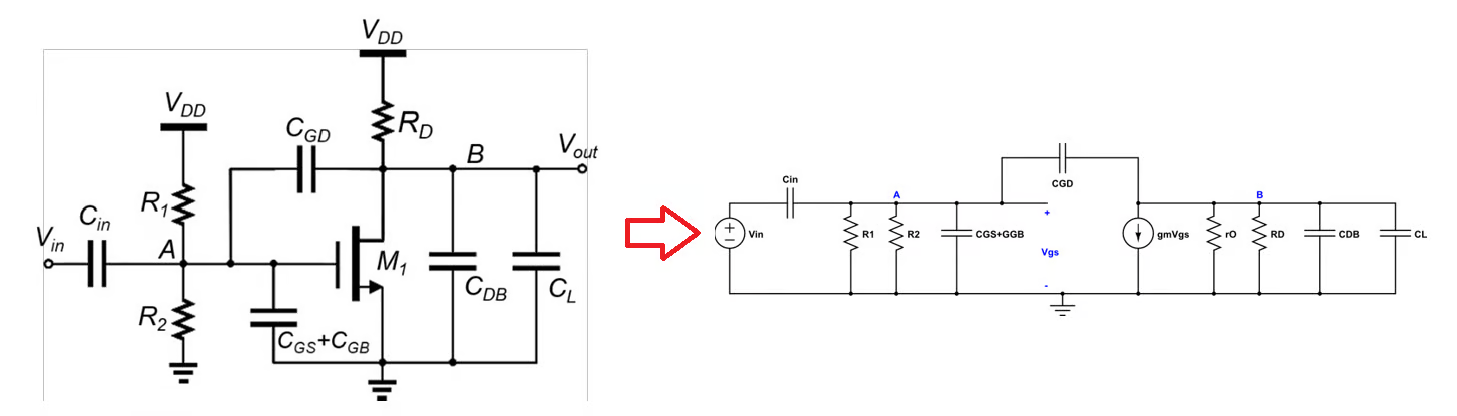
\includegraphics[width=1\linewidth]{images/final/5.png}
    \end{itemize}
    % TODO: Add the summary of the bode plot drawing into cheatsheet. Also include the info from Lec 10 recap that the magnitude bode plot always starts from the low-frequency voltage gain.
    % TODO: Add the inverting and non-inverting of the differential amplifier, this will help determine the starting point.
    \item (\textbf{Draw Bode Plot}): When draw a bode plot, the effect of poles and zeros should be \textbf{added} together. And the general poles and zeros roll-off table is shown below. \\
    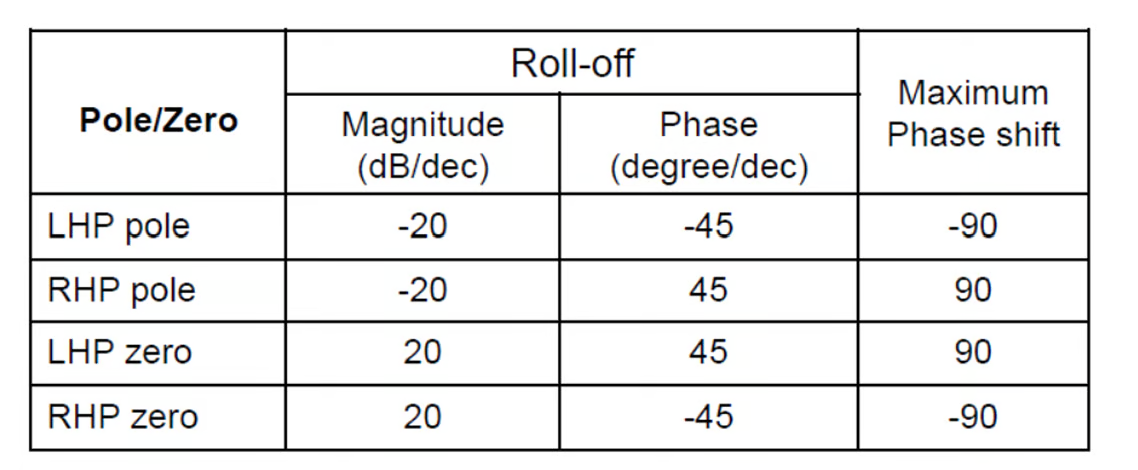
\includegraphics[width=1\linewidth]{images/final/6.png}
    \begin{itemize}
        \item For a normal pole or zero at $\omega_0$, the phase change occurs gradually from approximately $0.1\omega_0$ to $10\omega_0$. At $\omega_0$, the phase shift is approximately $\pm45^\circ$, and it approaches its full $\pm90^\circ$ shift by $10\omega_0$. Outside this range, there is no phase change.
        \item \textbf{Pole/Zero at the origin ($s=0$):} A \textbf{zero} contributes $+20\,\mathrm{dB/dec}$ and $+90^\circ$ phase, while a \textbf{pole} contributes $-20\,\mathrm{dB/dec}$ and $-90^\circ$ phase. Both apply at \textbf{all frequencies}.
        \begin{itemize}
            \item In a real amplifier circuit, \textbf{DC zero} is often accompanied by a low-frequency pole (e.g., due to a coupling capacitor). We can draw their \textbf{combined effect} directly in the magnitude Bode plot, rather than drawing their contributions separately. However, if the question gives a triangle black box, we should assume there is no low-frequency pole accompanying it!
            \item For a pole at origin, we should draw it explicitly in the magnitude bode plot.
        \end{itemize}
        \item For a \textbf{phase Bode plot}, there are several cases to consider when determining its starting phase:
        \begin{itemize}
            \item If the circuit is not an amplifier, normal zeros/poles start at $0^\circ$ and transition toward $+90^\circ/-90^\circ$ around their corner frequency. A zero/pole at the origin contributes $+90^\circ/-90^\circ$ at all frequencies, thus the starting point becomes $+90^\circ/-90^\circ$.
            \item If the circuit is an \textbf{inverting amplifier}, the phase plot will start at $180^\circ$. Otherwise, if it is a \textbf{non-inverting amplifier}, then the phase plot will start at $0^\circ$. If the amplifier has a DC zero, will add $90^\circ$ to the starting point.
        \end{itemize}
    \end{itemize}
    \item (\textbf{Calculation in magnitude bode plot}): We can use the following procedure to calculate the gain at different pole and zero frequencies using the magnitude Bode plot:
    \begin{itemize}
        \item Identify the \textbf{starting frequency and its corresponding gain}. Then, determine whether we need to find the gain at a given ending frequency or the ending frequency corresponding to a given gain.
        \item Based on the magnitude Bode plot we've drawn, identify the \textbf{slope between these two frequencies} (e.g., -20 or -40 dB/decade).
        \item Apply the following formula: $G_{\text{end}}=G_{\text{start}}+S\log_{10}\left(\frac{f_{\text{end}}}{f_{\text{start}}}\right)$, where G is the gain in dB and S is the slope in dB/decade (usually -20 or -40).
    \end{itemize}
    By substituting the known values, we can easily calculate the unknown gain or frequency!
    \item In a multiple-pole system, the \textbf{dominant pole} is the pole with the \textbf{lowest} pole frequency.
    \item The impedance $Z$ of a capacitor is $Z_C=\frac{1}{sC}$, e.g., if the voltage across a capacitor $C$ is $V$, then the current flowing through this capacitor will be $V\cdot sC$.
    \item From pole frequency $\omega$ to actual frequency $f$, $f=\frac{\omega}{2\pi}$.
    \item \textbf{Unit Conversion}: 
    $10^{9}$ (Giga, G);
    $10^{6}$ (Mega, M);
    $10^{3}$ (Kilo, k);
    $10^{2}$ (Hecto, h);
    $10^{1}$ (Deca, da);
    $10^{-1}$ (Deci, d);
    $10^{-2}$ (Centi, c);
    $10^{-3}$ (Milli, m);
    $10^{-6}$ (Micro, $\mu$);
    $10^{-9}$ (Nano, n);
    $10^{-12}$ (Pico, p);
    $10^{-15}$ (Femto, f);
    $10^{-18}$ (Atto, a);
    $10^{-21}$ (Zepto, z).
\end{enumerate}

\section{Current Mirrors}
\begin{enumerate}
    \item (\textbf{Basic Current Mirrors}): Assuming all transistors share the same $V_{GS}$ and operate in saturation, the output current is $I_{\text{OUT}}=\frac{(W/L)_{\text{OUT}}}{(W/L)_{\text{REF}}}I_{\text{REF}}$, neglecting channel-length modulation and device mismatch. \\
    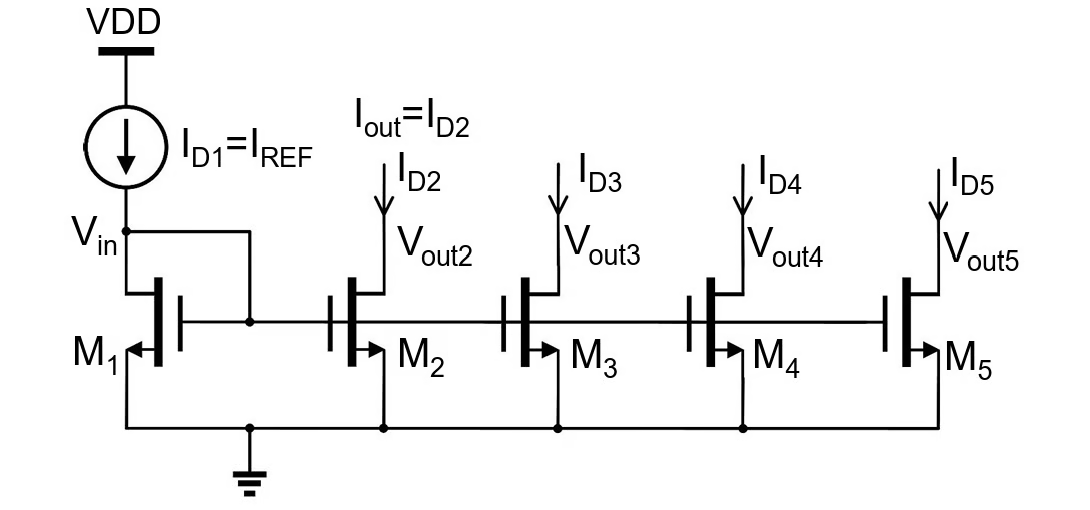
\includegraphics[width=1\linewidth]{images/final/7.png}
    \item (\textbf{System Error}): $\text{Err}\approx\lambda(V_{\text{out}}-V_{\text{in}})$. This error is caused by the CLM and the voltage difference between the reference transistor and the output transistor. Usually, no system error $\rightarrow V_{\text{in}}=V_{\text{out}}$.
    \item (\textbf{Random Error}): This is caused by fabrication errors, which might be resolved by redesigning the current mirror.
\end{enumerate}

\section{Differential Amplifier}
% TODO: Keep only one D-to-S differential amplifier. (the existing one suffices)
\begin{enumerate}
    \item (Two output normal differential amplifier with resistive load)
    \begin{itemize}
        \item The differential input is defined as $v_{i1}-v_{i2}$ and the differential output is defined as $v_{o2}-v_{o1}$ so that it's a \textbf{non-inverting amplifier}.
        \item (\textbf{Small signal Analysis}): In the small signal analysis, we have $v_{i1}=+\frac{v_{id}}{2}, v_{i2}=-\frac{v_{id}}{2}$ and the overall gain is $g_m(r_o||R_D)$.
        \item (\textbf{DC Operating Points}): The actual two inputs can be written as $v_{i1}=v_{ic}+\frac{v_{id}}{2}, v_{i2}=v_{ic}-\frac{v_{id}}{2}$, where $v_{ic}$ is the DC operating point that we need to find. In short, $v_{ic,\text{min}}=V_{GS1/2}+V_{OV3}$ where M3 is the MOSFET to implement the bias current source.
        \item (\textbf{Input and Output Swing}): Each half-end has a swing of $I_{SS}R_D$ ($I_{SS}$ is the current provided from the current source to the two branches). The total maximum output swing is $2I_{SS}R_D$. Thus, the maximum input range is $\frac{2I_{SS}R_D}{g_mR_D}=\frac{2I_{SS}}{g_m}$.
    \end{itemize}
    \item (DC/Systematic Offset Voltage)
    \begin{itemize}
        \item \textbf{Output offset}: Measure $V_{od}$ at $V_{id}=0$.
        \item \textbf{Input offset}: Measure $V_{id}$ at $V_{od}=0$.
        \item If we know one offset, it's very easy to calculate the other using the voltage gain. e.g., if we know $A_v$ and the output offset $V_o$, the input offset can be calculated as $\frac{V_o}{A_V}$.
    \end{itemize}
    \item (\textbf{Differential Pair with D-to-S Converter} (one output node): \\
    % TODO: Chaneg the tail current source from M7 to M5 by hand after printing
    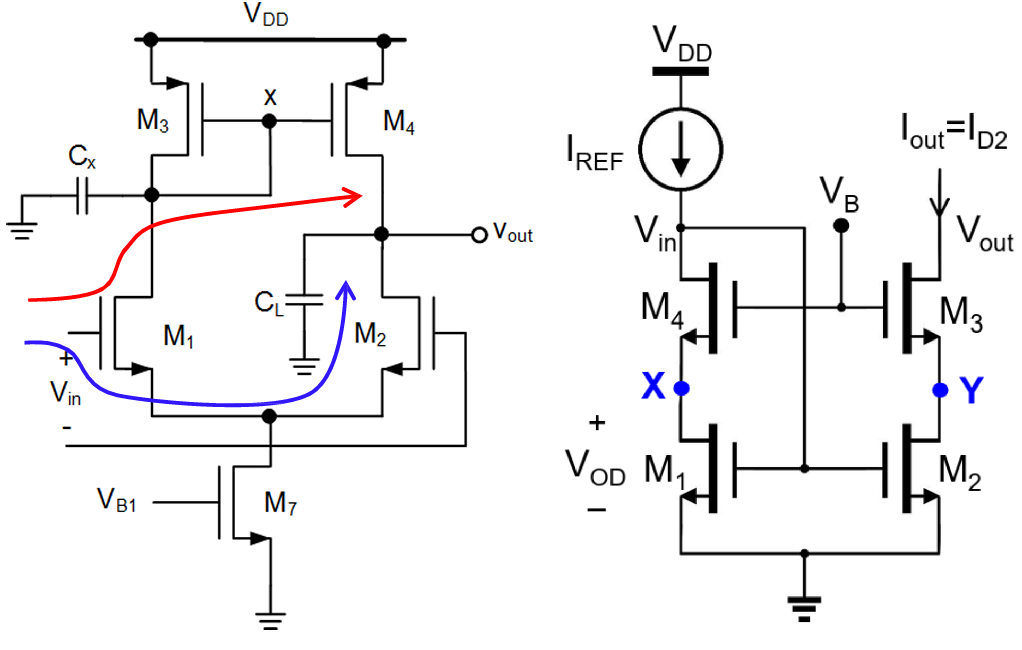
\includegraphics[width=1\linewidth]{images/final/8.png}
    \begin{itemize}
        \item (\textbf{Small Signal Analysis}): To find the voltage gain of any amplifier, we can use the following 4-step systemetic approach:
        \begin{itemize}
            \item Identify the number of signal paths from the inputs to the output: In this case, we have two, $v_{i2}\rightarrow v_{\text{out}}$ and $v_{i1}\rightarrow V_{X}\rightarrow v_{\text{out}}$.
            \item Determine how the signal paths interact: Following the definition of the input signal, $v_{id}=v_{i2}-v_{i1}$. Usually, we add the two signal paths together.
            \item Calculate the gain of each signal path: In this case, $v_{i2}\rightarrow v_{\text{out}}$, this is just a common-source amplifier, so we have $\frac{v_{out}}{v_{i2}}\approx-g_{m2}(r_{o2}\parallel r_{o4})$. Since we define $v_{i2}=\frac12v_{id}$, we have $A_{v1}\approx-\frac12g_{m2}(r_{o2}\parallel r_{o4})$. For the path $v_{i1}\rightarrow V_{X}\rightarrow v_{\text{out}}$, the first part is a CS amplifier with a diode-connected load and the second is a CS amplifier, thus, overall we have $\frac{v_{out}}{v_{i1}}\approx+g_{m1}(r_{o2}\parallel r_{o4})$ assuming M3 and M4 matches. Since we define $v_{i1}=-\frac12v_{id}$, we thus have $A_{v2}\approx-\frac12g_{m1}(r_{o2}\parallel r_{o4})$
            \item Calculate the overal gain: Use the relationship we've found in step 2. In this case, we \textbf{add} the two voltage gains, giving us $A_v\approx-g_m(r_{o2}\parallel r_{o4})$
        \end{itemize}
        \textbf{Note}: In a D-to-S differential amplifier, if we define $v_{id}=v_{i1}-v_{i2}$, we will have the overall voltage gain to be \textbf{positive}, which is $A_v=g_m(r_{o2}\parallel r_{o4})$!
        \item (\textbf{Frequency Response}): This amplifier has two signal paths, we should use get the transfer function for each path and then add them together to get the overal transfer function of this amplifier. This will give us two LHP poles $\frac{1}{r_{\text{out}}C_L}$, $\frac{g_{m3}}{C_x}$ and one LHP zero $\frac{2g_{m3}}{C_x}$!
    \end{itemize}
    \item (\textbf{Output Swing}): The maximum output voltage is usually $V_{DD}-V_{OV}$, while the minimum output voltage needs us to write the equation from $V_{DS}=V_{out,\text{min}}-V_{S}\geq V_{OV}$ and then derive the rest! If input common-mode signal is given, then $V_S$ should use the given input common-mode signal. Otherwise, we assume $V_S\geq V_{OV5}$ (the tail current source).
    \item (\textbf{Minimum Input DC Bias}): For an NMOS differential pair with an NMOS tail current source, the minimum input common-mode voltage is $V_{in,DC,\min}=V_{SS}+V_{OV,\text{tail}}+V_{THN}+V_{OV,\text{input}}$ where $V_{SS}$ is the voltage at the source of the current source! This applies to differential amplifiers, OTAs, and op-amps with this input topology. For PMOS input pair, $V_{IC,DC,\max}=V_{DD}-V_{OV,\text{tail}}-|V_{THP}|-V_{OV,\text{input}}$.
    \item (\textbf{The choice of $V_{OV}$}): For input NMOS, can be calculated using the expected voltage gain. For PMOS active load, choose $V_{OV}$ to satisfy the upper output swing requirement ($V_{out,\max}=V_{DD}-V_{OVP}$). For the tail current source, just randomly just a small number, like 0.3V.
    \item (\textbf{Differential Output Swing}): For a \textbf{fully differential amplifier} with balanced outputs, each output branch has half the specified differential output swing. For a \textbf{D-to-S differential amplifier}, the specified single-ended output swing applies directly to the output node (no division by 2).
    \item If we define our differential input as $v_{id}=v_{i2}-v_{i1}$, then in the small signal analysis, we shall use $v_{i2}=\frac12v_{id}$ and $v_{i1}=-\frac12v_{id}$
    \item (\textbf{Common-mode Gain}): It is defined as $A_{cm}=\frac{v_{o2}-v_{o1}}{v_{ic}}=\frac{v_{od}}{v_{ic}}$.
    \begin{itemize}
        \item In a two output normal differential amplifier ideally this should be zero, but the mismatch between the two halves of the amplifier makes this nonzero!
        \item In a D-to-S single output differential amplifier, even if both halves match, the common-mode gain is non-zero! It's $A_{cm,s}\approx-\frac{g_{m2}/g_{m3}}{1+2g_{m2}r_{o5}}$, where M1 and M2 are the input NMOS, M5 is the NMOS used to create the tail current and M3 and M4 are two PMOS current mirrors.
    \end{itemize}
    \item (\textbf{Common-mode Rejection Ratio}): It's defined as $\text{CMRR (dB)}=20\log_{10}\left|\frac{A_{vd}}{A_{cm}}\right|$ where $A_{vd}$ is the differential voltage gain!
    \item Pay attention to the load used at the differential amplifier!
\end{enumerate}

\section{Operational Amplifier}
\begin{enumerate}
    \item (\textbf{Two-stage Op-amp}):\\
    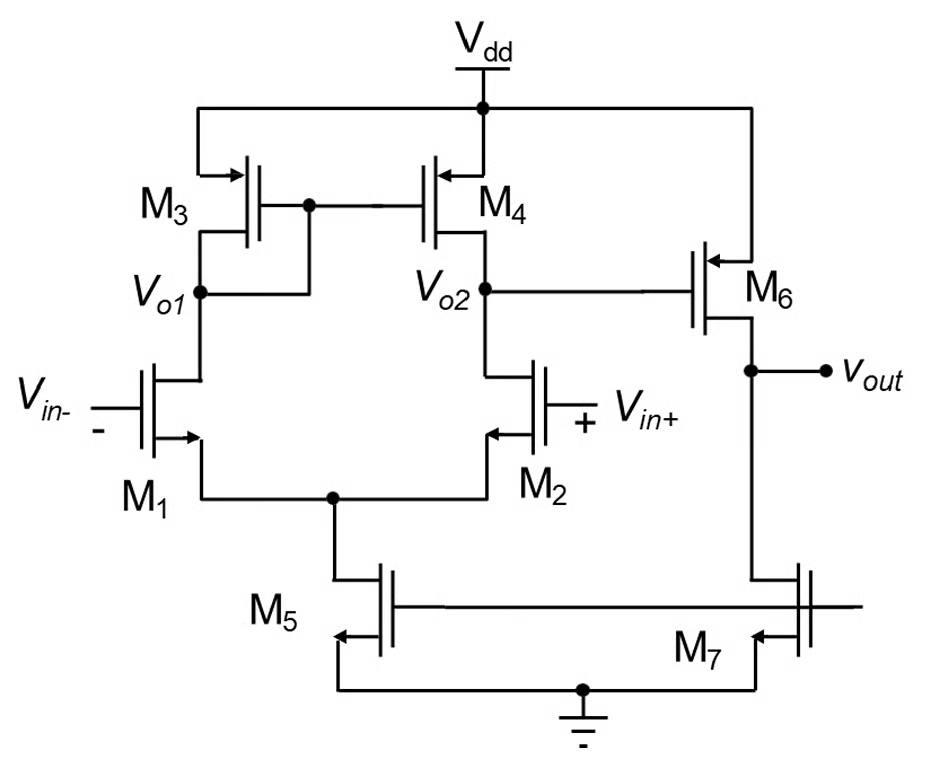
\includegraphics[width=1\linewidth]{images/final/9.png}
    \begin{itemize}
        \item \textbf{Small-Signal Analysis}: The gain is $g_{m1} g_{m6} (r_{o2} \parallel r_{o4})(r_{o7} \parallel r_{o6})$.
        \item \textbf{Output Swing}: $V_{DD}-V_{OV6}-V_{OV7}$.
        \item \textbf{Systematic Offset}: If $\frac{(W/L)_6}{(W/L)_3}=\frac{I_{D6}}{I_{D3}}$, then there is no systematic offset.
    \end{itemize}
    \textbf{Note}: In a D-to-S differential amplifier, we always have $V_{o1}=V_{o2}$ if we consider CLM!
    \item (\textbf{Telescopic Op-Amp}):\\
    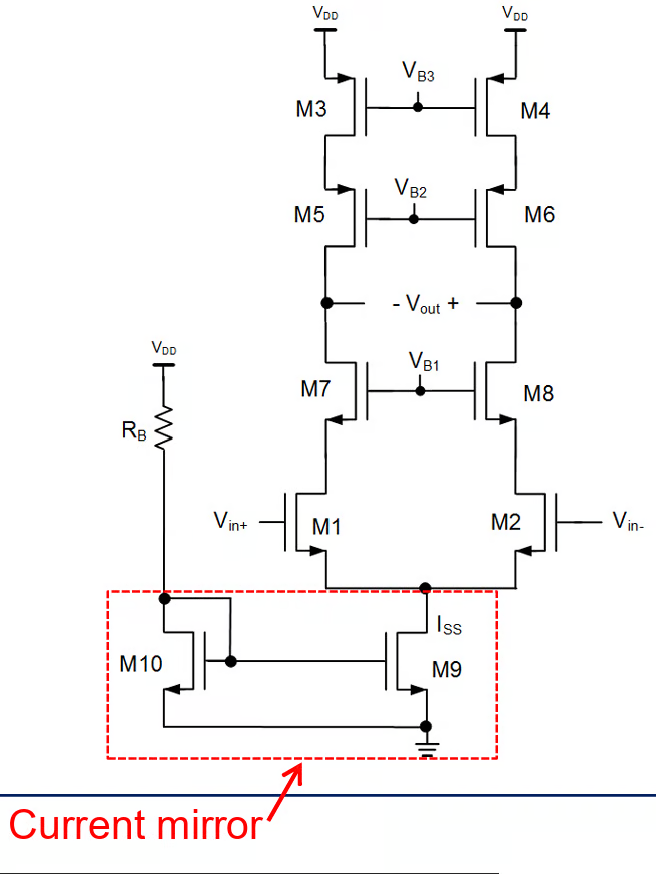
\includegraphics[width=1\linewidth]{images/final/10.png}
    \begin{itemize}
        \item \textbf{Small-signal Analysis}: The gain is $g_{m1}\left[(g_{m7}r_{o1}r_{o7})\parallel(g_{m5}r_{o3}r_{o5})\right]$
        \item \textbf{Output Swing}: $V_{\text{swing,diff}}=2V_{\text{swing}}=2V_{DD}-10|V_{OV}|$
        \item \textbf{DC Biasing}: $V_{B1}\le V_{THN}+V_{out,\min}$, where $V_{out,\min}=\frac{V_{DD}}2-3V_{OV} $. $V_{B2}\ge V_{out,\max}-|V_{THP}|$, where $V_{out,\max}=\frac{V_{DD}}2+2V_{OV}$. $V_{B3}\ge V_{D4,\max}-|V_{THP}|$ where $V_{D4,\max}=V_{B2}+V_{SG6}$ (after $V_{B2}$ is fixed). The idea of \textbf{worst-case analysis}: Consider the maximum or minimum node voltage that makes each transistor most likely to leave saturation.
    \end{itemize}
    \item (\textbf{Telescopic OTA with D-to-S converter}: The output swing becomes smaller $V_{sw}^+\le V_{DD}-V_{out}-(|V_{THP}|+2|V_{OV}|)$. $V_{sw}^-=V_{out}-3|V_{OV}|$, and $V_{\text{swing,diff}}=2\times\min(V_{sw}^+,V_{sw}^-)$.
\end{enumerate}

\section{Frequency Response Part 2}
\begin{enumerate}
    \item (\textbf{Open- and Closed-loop Amplifier}: \\
    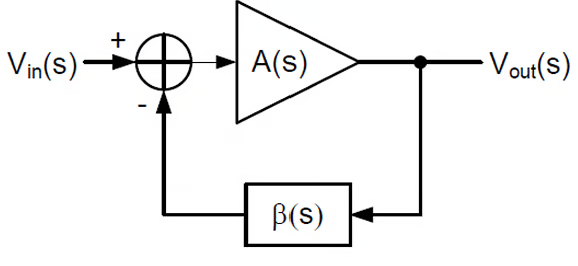
\includegraphics[width=1\linewidth]{images/final/11.png}
    $A(s)$ is the open-loop gain or open-loop transfer function. $\beta(s)$ is the feedback transfer function. $A(s)\beta(s)$ is the \textbf{loop gain}. The \textbf{closed-loop gain} is $\frac{V_{\text{out}}(s)}{V_{\text{in}}(s)}=\frac{A(s)}{1+A(s)\beta(s)}\approx\frac{1}{\beta(s)}$ (The approximation holds if the loop gain $A(s)\beta(s)\gg1$
    \item \textbf{Phase and Gain Margin}
    \begin{itemize}
        \item (\textbf{Gain Margin (GM)}): Measured at the frequency where the \textbf{loop-gain phase reaches $-180^\circ$}. It indicates how much the loop gain can increase before reaching $0\,\mathrm{dB}$. Thus, $\mathrm{GM}=0\,\mathrm{dB}-20\log_{10}|A(j\omega)\beta(j\omega)|\big|_{\angle A\beta=-180^\circ}$.
        \item (\textbf{Phase Margin (PM)}): Measured at the frequency where the \textbf{loop-gain magnitude reaches $0\,\mathrm{dB}$} (unity-gain frequency). It indicates how much additional phase lag can be introduced before reaching $-180^\circ$. Thus, $\mathrm{PM}=180^\circ+\angle A(j\omega)\beta(j\omega)\big|_{|A\beta|=1}$.
    \end{itemize}
    \item (\textbf{Frequency Response of an OTA}):\\
    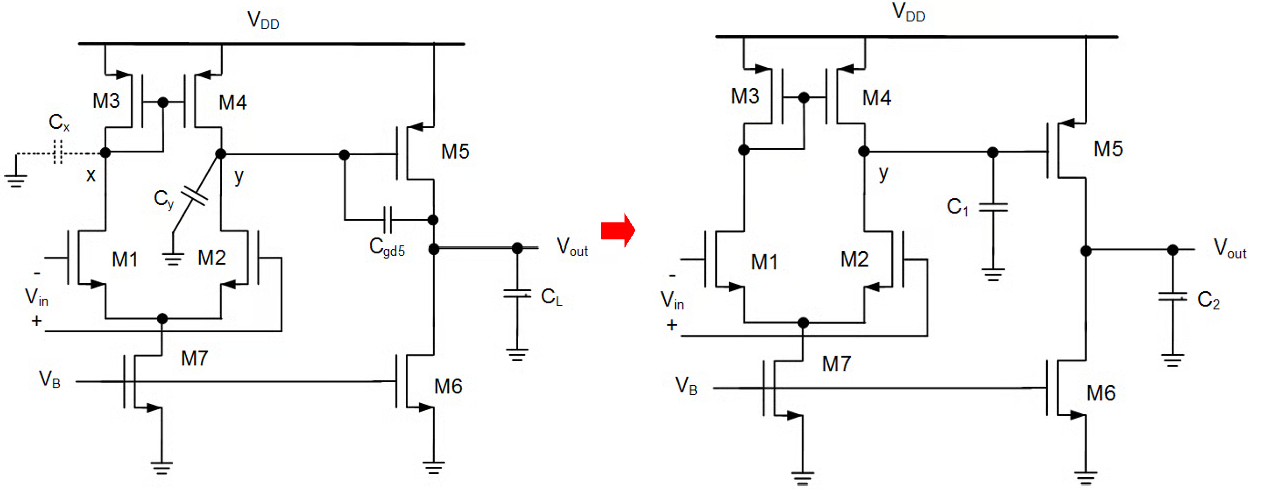
\includegraphics[width=1\linewidth]{images/final/12.png}
    \begin{itemize}
        \item \textbf{Initial}: We ignore the 1 pole and 1 zero associated with node X. The transfer function is $\frac{V_{\text{out}}(s)}{V_{\text{in}}(s)} \approx\frac{g_{m2}R_1g_{m5}R_2(1-s/\omega_z)}{(1+s/\omega_{p1})(1+s/\omega_{p2})}$, where $\omega_{p1}\approx\frac{1}{R_1C_1}, \omega_{p2}\approx\frac{1}{R_2C_2}, \omega_z\approx\frac{g_{m5}}{C_{gd5}}$, $C_1=C_y+(1+A_{v2})C_{gd5}, C_2=C_L+C_{gd5}$ ($A_{v2}$ is the magnitude of the voltage gain of the second-stage CS amplifier), $R_1=r_{o2}\parallel r_{o4}, R_2=r_{o5}\parallel r_{o6}$
        \item \textbf{After pole splitting}: We repalce $C_{gd5}$ with a larger $C_c$. We have the dominant pole $\omega_{p1}\approx\frac{1}{(r_{o2}\parallel r_{o4})[1+g_{m5}(r_{o5}\parallel r_{o6})]C_c}$, non-dominant pole $\omega_{p2}\approx\frac{g_{m5}C_c}{C_yC_L+C_cC_y+C_cC_L}$ and the zero $\omega_z\approx\frac{g_{m5}}{C_c}$.
        \item \textbf{After pole splitting + lead compensation}: We connect a resistor in seris with $C_c$, our zero becomes $\omega_z=s_z=\frac{1}{C_c\left(\frac{1}{g_{m5}}-R_c\right)}$. The ideal value for $R_c$ is $R_c\approx\frac{1}{g_{m5}}\left(\frac{C_c+C_L}{C_c}\right)$, which is when $\omega_{p2}=\omega_z$
    \end{itemize}
    \item (\textbf{Unity Gain Bandwidth}): The frequency at which the gain magnitude reaches 0 dB (unity), the unit is in rad/s. $\left|\frac{V_{\text{out}}(j\omega)}{V_{\text{in}}(j\omega)}\right|=\frac{A_v}{\sqrt{1+\left(\frac{\omega_u}{\omega_{3\text{dB}}}\right)^2}}=1$. If $\omega_u\gg\omega_{3\text{dB}}$, we have $\omega_u\approx A_v\omega_{3\text{dB}}\text{ or }f_u\approx A_vf_{3\text{dB}}$. For example, in the OTA bullet point above, $\omega_u=A_v\omega_{p1}\approx\frac{g_{m2}}{C_C}$.
    \item (\textbf{Frequency Response of a Telescope Op-amp}): The dominant pole is $\omega_{p1}\approx\frac{1}{r_{\text{out}}C_L}$, the rest are at much higher frequencies. So, the unit-gain frequency is $\omega_u\approx A_v\omega_{p1} =\frac{g_{m2}r_{\text{out}}}{r_{\text{out}}C_L}=\frac{g_{m2}}{C_L}$.
\end{enumerate}

\end{multicols}

% Dividing Line
% \hrulefill \\
% \begin{multicols}{4}
% \begin{enumerate}
% \end{enumerate}
% \end{multicols}

\end{document}